\section{Results}
\label{sec:results}

\subsection{The bias of the holdout estimate}

Table~\ref{tab:main-results} gives the main comparison. Under the protocol the holdout AUC of the WoE scorecard has a bias of \nv{syn.w.none.bias}$\,\pm\,$\nv{syn.w.none.ci} against the reference sample, a root mean squared error of \nv{syn.w.none.rmse}, and the 95\% interval of the engine covers the reference value in \nv{syn.w.none.cov}\% of the \nv{syn.reps} repetitions (Wilson interval \nv{syn.w.none.covlo} to \nv{syn.w.none.covhi}\%). The standardised logit has a bias of \nv{syn.l.none.bias}$\,\pm\,$\nv{syn.l.none.ci} and a coverage of \nv{syn.l.none.cov}\%. The same holds in the other three settings of Table~\ref{tab:other-data}: on \nv{small.n} rows the bias is \nv{small.w.none.bias}$\,\pm\,$\nv{small.w.none.ci} with a coverage of \nv{small.w.none.cov}\%, on the card holders \nv{tw.w.none.bias}$\,\pm\,$\nv{tw.w.none.ci} with \nv{tw.w.none.cov}\%, and for the product's own scorecard \nv{prod.p.none.bias}$\,\pm\,$\nv{prod.p.none.ci} with \nv{prod.p.none.cov}\% (Wilson interval \nv{prod.p.none.covlo} to \nv{prod.p.none.covhi}\%). In all six cells of the two models and three data sets the interval of the bias contains zero and the interval of the coverage contains 0.95, so that the first prediction holds and Proposition~\ref{prop:unbiased} is borne out. The calibration error is the exception: its bias under the protocol is \nv{syn.w.none.ece} for the scorecard, because the average of the absolute differences over ten groups of 75 rows is positive even for a perfectly calibrated model, while the reference rows, 50,000 of them, make it nearly zero; it is a property of the estimator of the calibration error at this holdout size and not of the protocol. The Brier score has a second small exception: its bias under the protocol is negative on the small sample (\nv{small.w.none.brier}$\,\pm\,$\nv{small.w.none.brierci}) and on the card holders (\nv{tw.w.none.brier}$\,\pm\,$\nv{tw.w.none.brierci}), with an interval that excludes zero, so that the holdout scores a little better than the reference sample. A plausible cause, not tested here, is that the stratified holdout shares the event share on which the intercept of the model was fitted, while each reference sample is drawn afresh; the size is smaller than the Brier effect of the calibration leak (\nv{syn.w.caltest.brier}).

\begin{table*}[htbp]
\centering
\small
\caption{Bias of the holdout estimate of the AUC, the Brier score and the calibration error against the value on a reference sample of 50,000 rows that no step read, for the proposed protocol and for each leaked variant, on 300 planted data sets of 2,500 rows with 40 inputs; the coverage column is the share of the 95\% intervals of the engine's AUC variance that contain the reference value. The two five-fold rows compare the cross-validated AUC with the mean reference AUC of the fold models.}
\label{tab:main-results}
\fitwidth{%
\begin{tabular}{llrrrrr}
\toprule
Model & Validation procedure & AUC bias $\pm$ 95\% half-width & RMSE & Coverage \% [Wilson 95\%] & Brier bias & ECE bias \\
\midrule
WoE scorecard & proposed protocol & $0.000\pm0.002$ & 0.018 & 95.3 [92, 97] & $-0.0001\pm0.0008$ & $+0.0148\pm0.0014$ \\
 & imputation on all rows & $0.000\pm0.002$ & 0.018 & 95.3 [92, 97] & $0.0000\pm0.0008$ & $+0.0145\pm0.0014$ \\
 & bin edges on all rows & $-0.001\pm0.002$ & 0.018 & 96.3 [94, 98] & $+0.0001\pm0.0008$ & $+0.0147\pm0.0014$ \\
 & WoE with holdout labels & $+0.018\pm0.002$ & 0.026 & 78.3 [73, 83] & $-0.0062\pm0.0008$ & $+0.0126\pm0.0014$ \\
 & screen with holdout labels & $+0.004\pm0.002$ & 0.019 & 94.3 [91, 96] & $-0.0016\pm0.0008$ & $+0.0132\pm0.0013$ \\
 & everything fitted on training and holdout & $+0.025\pm0.002$ & 0.032 & 66.7 [61, 72] & $-0.0088\pm0.0009$ & $+0.0113\pm0.0014$ \\
 & configuration chosen on the holdout & $+0.005\pm0.002$ & 0.018 & 96.0 [93, 98] & $-0.0018\pm0.0008$ & $+0.0127\pm0.0013$ \\
 & calibration map fitted on the holdout & $+0.016\pm0.002$ & 0.023 & 88.0 [84, 91] & $-0.0081\pm0.0007$ & $-0.0055\pm0.0011$ \\
 & calibration slice overlapping the holdout & $+0.004\pm0.002$ & 0.018 & 94.3 [91, 96] & $-0.0022\pm0.0008$ & $+0.0113\pm0.0014$ \\
 & five-fold, preprocessing inside the folds & $-0.001\pm0.002$ & 0.015 & -- & -- & -- \\
 & five-fold, preprocessing before the folds & $+0.054\pm0.001$ & 0.055 & -- & -- & -- \\
standardised logit & proposed protocol & $-0.001\pm0.002$ & 0.017 & 94.7 [92, 97] & $+0.0002\pm0.0008$ & $+0.0150\pm0.0012$ \\
 & imputation on all rows & $-0.001\pm0.002$ & 0.017 & 94.3 [91, 96] & $+0.0002\pm0.0008$ & $+0.0142\pm0.0013$ \\
 & scaling on all rows & $-0.001\pm0.002$ & 0.017 & 95.0 [92, 97] & $+0.0002\pm0.0008$ & $+0.0149\pm0.0012$ \\
 & screen with holdout labels & $+0.004\pm0.002$ & 0.017 & 93.7 [90, 96] & $-0.0017\pm0.0008$ & $+0.0130\pm0.0012$ \\
 & everything fitted on training and holdout & $+0.009\pm0.002$ & 0.019 & 92.7 [89, 95] & $-0.0034\pm0.0008$ & $+0.0118\pm0.0013$ \\
 & configuration chosen on the holdout & $-0.001\pm0.002$ & 0.017 & 95.0 [92, 97] & $+0.0002\pm0.0008$ & $+0.0150\pm0.0013$ \\
 & calibration map fitted on the holdout & $+0.014\pm0.002$ & 0.021 & 87.0 [83, 90] & $-0.0079\pm0.0007$ & $-0.0063\pm0.0011$ \\
 & calibration slice overlapping the holdout & $+0.003\pm0.002$ & 0.017 & 96.0 [93, 98] & $-0.0019\pm0.0007$ & $+0.0109\pm0.0012$ \\
 & five-fold, preprocessing inside the folds & $-0.001\pm0.001$ & 0.012 & -- & -- & -- \\
 & five-fold, preprocessing before the folds & $+0.005\pm0.001$ & 0.013 & -- & -- & -- \\
\bottomrule
\end{tabular}%
}
\end{table*}


Figure~\ref{fig:bias-by-leak} shows the AUC bias of every variant with its interval, for both models and two sample sizes. Three groups appear. The first group reads only holdout inputs: imputation on all rows, scaling on all rows and bin edges on all rows. On the planted data their biases are \nv{syn.w.imp.bias} (imputation) and \nv{syn.w.bin.bias} (bin edges) for the scorecard and \nv{syn.l.imp.bias} (imputation) and \nv{syn.l.scale.bias} (scaling) for the logit, all within the half-width of the protocol, and the same holds on the small sample and the card holders, so that the prediction that these steps leave the estimate within 0.005 of the truth holds in all twelve cells. The second group reads holdout labels. The weight of evidence computed with the holdout labels adds \nv{syn.w.woe.bias}$\,\pm\,$\nv{syn.w.woe.ci} to the AUC of the scorecard and lowers the coverage to \nv{syn.w.woe.cov}\%; fitting every step on the training slice and the holdout adds \nv{syn.w.fit.bias}$\,\pm\,$\nv{syn.w.fit.ci}, and the coverage falls to \nv{syn.w.fit.cov}\%. The logit, whose steps are less flexible, gains less: \nv{syn.l.fit.bias} with a coverage of \nv{syn.l.fit.cov}\%. The third group is the calibration: a map fitted on the holdout adds \nv{syn.w.caltest.bias}$\,\pm\,$\nv{syn.w.caltest.ci} to the AUC of the scorecard and \nv{syn.l.caltest.bias} to that of the logit, lowers the Brier score by \nv{syn.w.caltest.brier} and turns the bias of the calibration error from \nv{syn.w.none.ece} to \nv{syn.w.caltest.ece}: the model looks better calibrated than it is, and by a margin that is of the order of the whole error. A calibration slice that overlaps the holdout in a fifth of its rows adds \nv{syn.w.calov.bias} to the AUC, in proportion to the overlap.

\begin{figure}[htbp]
\centering
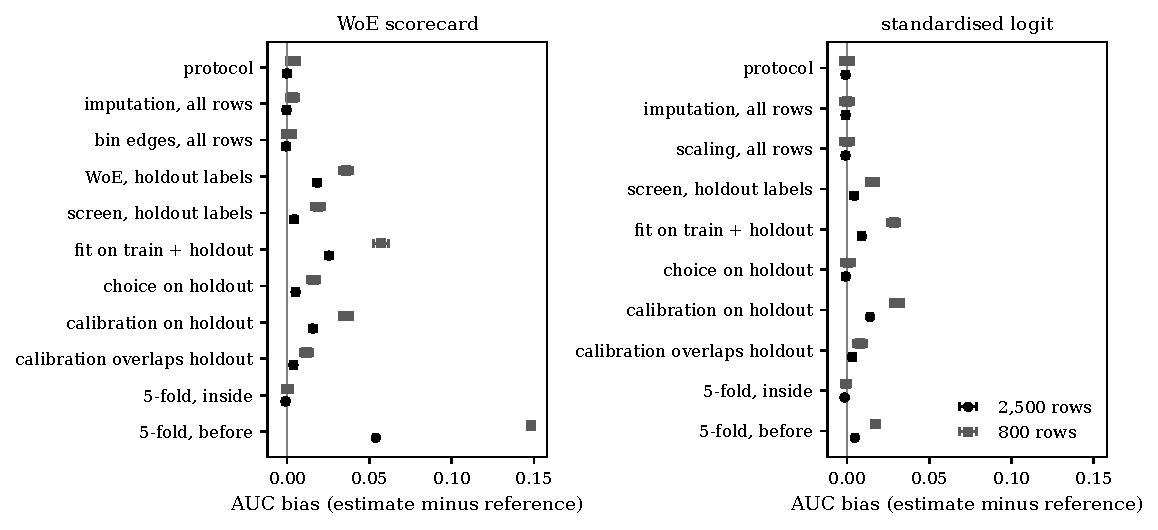
\includegraphics[width=\textwidth]{figures/fig-bias-by-leak.pdf}
\caption{Bias of the holdout AUC, the estimate minus the value of the same fitted model on the reference sample, with its 95\% half-width over repetitions, for the protocol and for every leaked variant, for the WoE scorecard (left) and the standardised logit (right) on planted data of 2,500 rows (circles) and of 800 rows (squares).}
\label{fig:bias-by-leak}
\end{figure}

The choice of a configuration on the holdout has a small cost. The scorecard chooses among eight configurations and its bias is \nv{syn.w.sel.bias}$\,\pm\,$\nv{syn.w.sel.ci} on the planted data and \nv{small.w.sel.bias} on the small sample; the logit chooses between two and its bias is \nv{syn.l.sel.bias} and \nv{small.l.sel.bias}. This is the pattern of Proposition~\ref{prop:selection}: with configurations that are strongly correlated the optimism is a small fraction of the bound $\sigma\sqrt{2\ln K}$, and it grows with $K$ and with the smaller holdout. The two five-fold procedures separate cleanly. Preprocessing inside the folds gives a bias of \nv{syn.w.cvin.bias}$\,\pm\,$\nv{syn.w.cvin.ci}; preprocessing on all development rows before the folds gives \nv{syn.w.cvpre.bias}$\,\pm\,$\nv{syn.w.cvpre.ci} on the planted data and \nv{small.w.cvpre.bias}$\,\pm\,$\nv{small.w.cvpre.ci} on the small sample, an optimism larger than that of every holdout leak on the planted data, because the binning, the weight of evidence and the screen of every fold were fitted with the validation rows of that fold. The logit, whose screen is a correlation that keeps ten of 40 inputs and which has no weight of evidence, gains less: \nv{syn.l.cvpre.bias} on the planted data and \nv{tw.l.cvpre.bias}$\,\pm\,$\nv{tw.l.cvpre.ci} on the card holders, where the interval contains zero.

\begin{figure}[htbp]
\centering
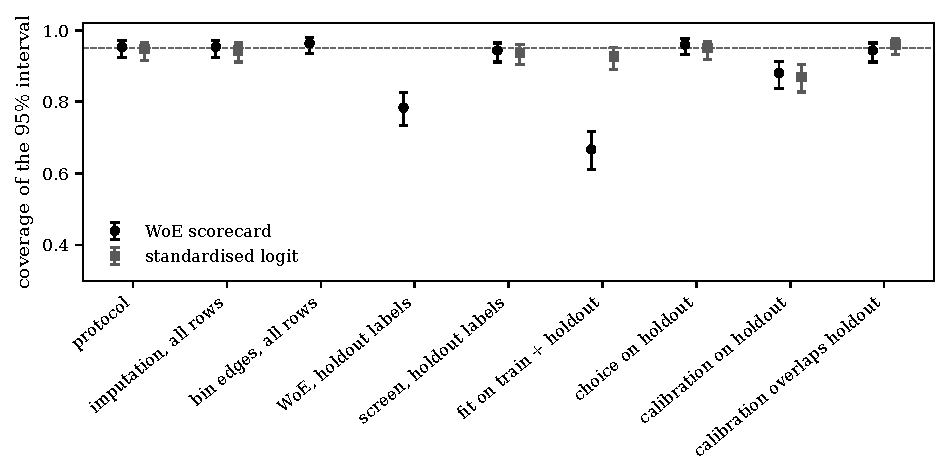
\includegraphics[width=\textwidth]{figures/fig-coverage.pdf}
\caption{Coverage of the engine's 95\% interval of the holdout AUC, the share of 300 repetitions in which the interval contains the reference value of the fitted model, for the WoE scorecard (circles) and the standardised logit (squares) on planted data of 2,500 rows, with Wilson intervals; the dotted line is the nominal 0.95.}
\label{fig:coverage}
\end{figure}

Figure~\ref{fig:coverage} shows what the leaks do to the interval that a validator reports. The leaks that read labels do not only move the point estimate: they leave the interval where it was, so that it fails to cover the reference value. For the scorecard the coverage falls to \nv{syn.w.woe.cov}\% for the weight of evidence with holdout labels, \nv{syn.w.fit.cov}\% for the fit on everything and \nv{syn.w.caltest.cov}\% for the calibration on the holdout, and for the product's own scorecard fitted on everything to \nv{prod.p.fit.cov}\% (Wilson interval \nv{prod.p.fit.covlo} to \nv{prod.p.fit.covhi}\%). A validator that reads the interval as a statement about the future is therefore misled by more than the point estimate suggests. Figure~\ref{fig:bias-distribution} gives the distribution of the bias in a repetition: the protocol is centred on zero with the spread of the sampling error of the holdout, and the leaked variants are the same distribution shifted to the right.

\begin{figure}[htbp]
\centering
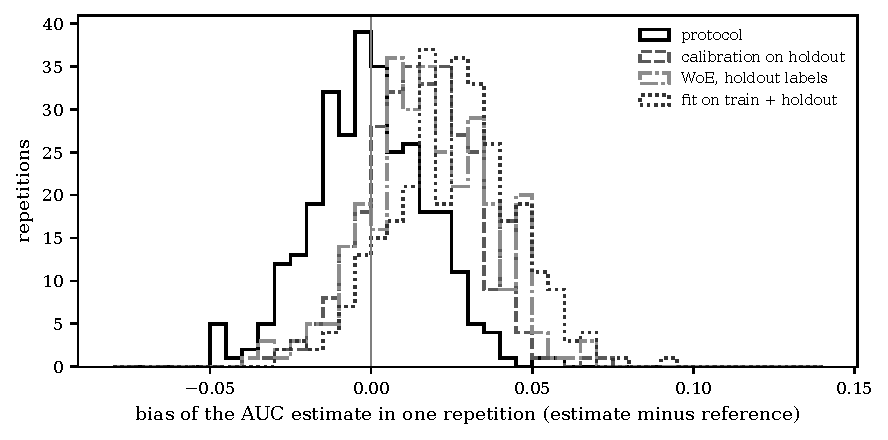
\includegraphics[width=0.85\textwidth]{figures/fig-bias-distribution.pdf}
\caption{Distribution over 300 repetitions of the bias of the holdout AUC in one repetition for the WoE scorecard on planted data of 2,500 rows: the protocol and three leaked variants, drawn as step histograms of the estimate minus the reference value of the fitted model.}
\label{fig:bias-distribution}
\end{figure}

\begin{table*}[htbp]
\centering
\small
\caption{Bias of the holdout AUC (with its 95\% half-width) and coverage of the 95\% interval in percent for the WoE scorecard on planted data of 800 rows (300 repetitions), on the 2,500-row subsamples of the 30,000 card holders of C01 (150 repetitions, 10,000 rows set aside per repetition as the reference), and for the product's own optbinning scorecard on planted data (90 repetitions; only the variants that call the product's fit appear).}
\label{tab:other-data}
\fitwidth{%
\begin{tabular}{lrrrrrr}
\toprule
Validation procedure & Small sample bias & Cov. & Card holders bias & Cov. & Product scorecard bias & Cov. \\
\midrule
proposed protocol & $+0.003\pm0.004$ & 95 & $+0.002\pm0.004$ & 93 & $+0.001\pm0.004$ & 93 \\
imputation on all rows & $+0.003\pm0.004$ & 95 & $+0.002\pm0.004$ & 93 & -- & -- \\
bin edges on all rows & $+0.001\pm0.004$ & 93 & $+0.002\pm0.004$ & 94 & -- & -- \\
WoE with holdout labels & $+0.036\pm0.004$ & 72 & $+0.015\pm0.004$ & 88 & -- & -- \\
screen with holdout labels & $+0.019\pm0.004$ & 89 & $+0.003\pm0.004$ & 93 & -- & -- \\
everything fitted on training and holdout & $+0.057\pm0.004$ & 54 & $+0.019\pm0.004$ & 85 & $+0.039\pm0.004$ & 36 \\
configuration chosen on the holdout & $+0.016\pm0.004$ & 91 & $+0.004\pm0.004$ & 94 & -- & -- \\
calibration map fitted on the holdout & $+0.036\pm0.004$ & 80 & $+0.020\pm0.004$ & 81 & $+0.016\pm0.004$ & 81 \\
calibration slice overlapping the holdout & $+0.012\pm0.004$ & 93 & $+0.007\pm0.004$ & 91 & -- & -- \\
five-fold, preprocessing inside the folds & $+0.000\pm0.003$ & -- & $+0.001\pm0.003$ & -- & -- & -- \\
five-fold, preprocessing before the folds & $+0.148\pm0.002$ & -- & $+0.016\pm0.003$ & -- & -- & -- \\
\bottomrule
\end{tabular}%
}
\end{table*}


Table~\ref{tab:other-data} shows that the pattern holds on the other data. On the small sample the effects are about twice as large, as the sampling noise that the leaked step fits is larger: the fit on everything adds \nv{small.w.fit.bias}$\,\pm\,$\nv{small.w.fit.ci} with a coverage of \nv{small.w.fit.cov}\%. On the card holders the effects are smaller (\nv{tw.w.fit.bias} for the fit on everything, \nv{tw.w.woe.bias} for the weight of evidence, \nv{tw.w.caltest.bias} for the calibration on the holdout), except that of the calibration, which is as large as on the planted data; the card holders have 20 inputs against 40, and the cross-validation results below show that the optimism of a leak that fits noise grows with the number of inputs. The screen with holdout labels adds \nv{tw.w.scr.bias}$\,\pm\,$\nv{tw.w.scr.ci} on the card holders, which is not distinguishable from zero. The second prediction required the three label-reading steps to inflate the AUC on every data set; it holds on the planted data (three of three) and on the small sample (three of three) and fails on the card holders (two of three), and it is reported as not held. The product's scorecard fitted on everything adds \nv{prod.p.fit.bias}$\,\pm\,$\nv{prod.p.fit.ci} and its calibration on the holdout \nv{prod.p.caltest.bias}$\,\pm\,$\nv{prod.p.caltest.ci}, so that the compact pipeline and the product's fit give the same sign and the same order of magnitude; the product's scorecard, whose binning is the optimal binning of its package, gains more from the fit on everything (\nv{prod.p.fit.bias} against \nv{syn.w.fit.bias}) and the same from the calibration on the holdout.

\subsection{What the gates detect}

Table~\ref{tab:gates} and Figure~\ref{fig:gate-matrix} give the share of \nv{e2.reps} draws in which each gate fails, for the leaks planted in the fitting path. On the protocol no gate fails in any draw, for either model, and the non-vacuity control is satisfied in every draw; with zero failures in \nv{e2.reps} draws, the Wilson upper bound of the false-alarm rate is \nv{e2.fa.upper}\%. The three gates are complementary. The first gate (transforms on the training slice only) fails in every draw for every leak that reads holdout rows in a transform (imputation, scaling, bin edges, weight of evidence, screen and the fit on everything), and it is blind to the calibration leaks (0\% for both). The second gate (calibration slice disjoint and invariant to the holdout labels) fails in every draw for the leaks that read labels and for the calibration leaks and, through the calibration map that depends on the chosen configuration, in \nv{e2.w.sel.G2}\% and \nv{e2.l.sel.G2}\% of the draws for the choice on the holdout (scorecard and logit); it is blind to the input-only leaks, imputation, scaling and bin edges (0\%). The third gate fails for every leak that the first two catch, except that against the choice on the holdout it has the power of Proposition~\ref{prop:discrete}.

\begin{table}[htbp]
\centering
\small
\caption{Share of 100 data draws of 1,500 rows in which each gate fails, so that the leak is detected: G1 moves the inputs outside the training slice, G2 requires disjoint slices and a calibration map unchanged when the holdout labels are flipped, G3 perturbs the holdout inputs and labels (one perturbation draw) and requires every fitted parameter unchanged. The first row of each model is the proposed protocol, where a failure is a false alarm.}
\label{tab:gates}
\fitwidth{%
\begin{tabular}{llrrrr}
\toprule
Model & Leak planted in the fitting path & G1 & G2 & G3 & Any gate \\
\midrule
WoE scorecard & none (false alarm rate) & 0 & 0 & 0 & 0 \\
 & imputation on all rows & 100 & 0 & 100 & 100 \\
 & bin edges on all rows & 100 & 0 & 100 & 100 \\
 & WoE with holdout labels & 100 & 100 & 100 & 100 \\
 & screen with holdout labels & 100 & 100 & 100 & 100 \\
 & everything fitted on training and holdout & 100 & 100 & 100 & 100 \\
 & configuration chosen on the holdout & 92 & 100 & 91 & 100 \\
 & calibration map fitted on the holdout & 0 & 100 & 100 & 100 \\
 & calibration slice overlapping the holdout & 0 & 100 & 100 & 100 \\
standardised logit & none (false alarm rate) & 0 & 0 & 0 & 0 \\
 & imputation on all rows & 100 & 0 & 100 & 100 \\
 & scaling on all rows & 100 & 0 & 100 & 100 \\
 & screen with holdout labels & 100 & 100 & 100 & 100 \\
 & everything fitted on training and holdout & 100 & 100 & 100 & 100 \\
 & configuration chosen on the holdout & 50 & 99 & 48 & 100 \\
 & calibration map fitted on the holdout & 0 & 100 & 100 & 100 \\
 & calibration slice overlapping the holdout & 0 & 100 & 100 & 100 \\
\bottomrule
\end{tabular}%
}
\end{table}


\begin{figure}[htbp]
\centering
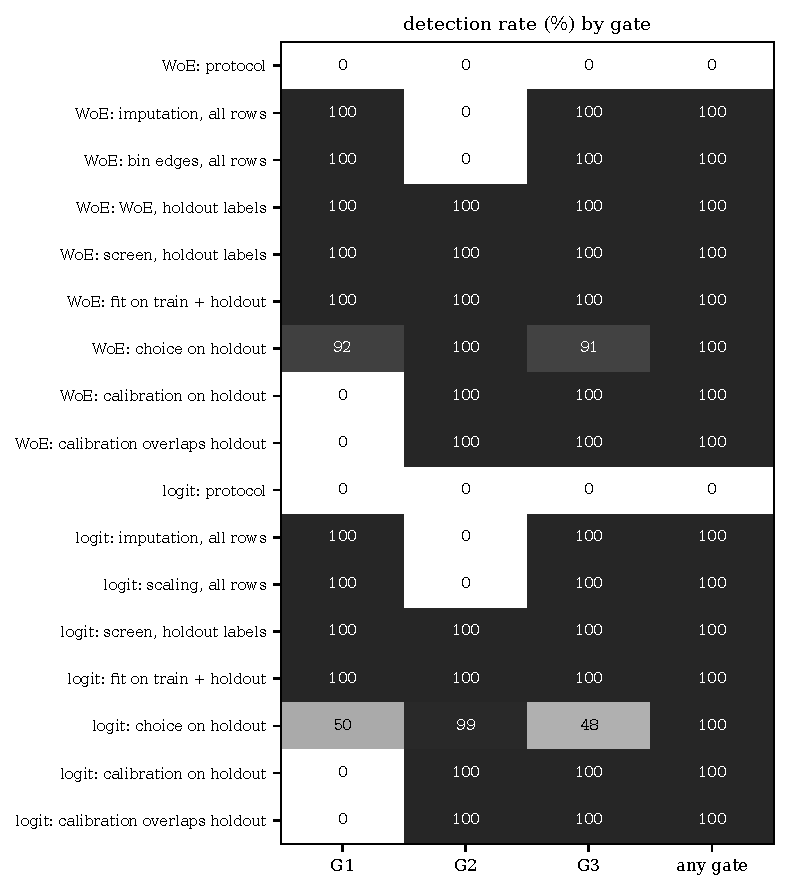
\includegraphics[width=0.62\textwidth]{figures/fig-gate-matrix.pdf}
\caption{Detection rate in percent of the three gates and of any of them for each leak planted in the fitting path of the WoE scorecard and of the standardised logit, over 100 draws of 1,500 rows; the first row of each model is the protocol, where a detection would be a false alarm.}
\label{fig:gate-matrix}
\end{figure}

At least one gate fails for every one of the \nv{h5.total} leaks in every draw (minimum over leaks \nv{h5.minany}\%) and none fails on the protocol, so that the fifth prediction holds. The leaks that read only holdout inputs are the instructive ones: the gates fail on them in every draw although their bias in Table~\ref{tab:main-results} is nil. A failure of a gate says that a rule was broken, not that the estimate is wrong; the bias that the rule protects against depends on the step, and the gates cannot tell a harmless breach from a harmful one. The choice of a configuration on the holdout is the case in which the third gate is partial: it fails in \nv{e2.w.sel.G3}\% of the draws for the scorecard, which chooses among eight configurations, and in \nv{e2.l.sel.G3}\% for the logit, which chooses between two. Figure~\ref{fig:detection-draws} (left) shows how repeating the perturbation raises the detection: with one, two, three and five draws the scorecard's choice is detected in \nv{e2.draws.w.1}, \nv{e2.draws.w.2}, \nv{e2.draws.w.3} and \nv{e2.draws.w.5}\% of \nv{e2.draws.reps} draws, against \nv{e2.draws.pred.w.1}, \nv{e2.draws.pred.w.2}, \nv{e2.draws.pred.w.3} and \nv{e2.draws.pred.w.5}\% for $1-K^{-d}$, and the logit's in \nv{e2.draws.l.1}, \nv{e2.draws.l.2}, \nv{e2.draws.l.3} and \nv{e2.draws.l.5}\% against \nv{e2.draws.pred.l.1}, \nv{e2.draws.pred.l.2}, \nv{e2.draws.pred.l.3} and \nv{e2.draws.pred.l.5}\%; the simulation has a standard error of up to \nv{e2.draws.se} points, and every observed rate is within \nv{e2.draws.zmax} standard errors of the prediction, each taken at its own predicted rate.

\begin{figure}[htbp]
\centering
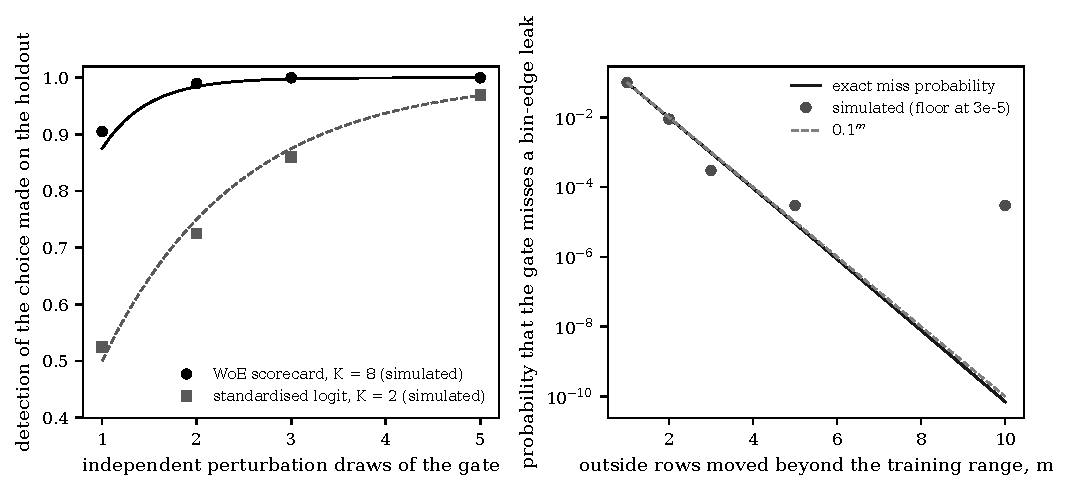
\includegraphics[width=\textwidth]{figures/fig-detection-draws.pdf}
\caption{Left: detection by the third gate of a choice made on the holdout, against the number of independent perturbation draws, for the scorecard (eight configurations) and the logit (two) in 200 draws of the data, with the curves $1-K^{-d}$ of Proposition~\ref{prop:discrete}. Right: probability that the gate misses a leak through a bin edge against the number of outside rows moved, simulated, exact (Proposition~\ref{prop:detection}) and $0.1^m$.}
\label{fig:detection-draws}
\end{figure}

\begin{table}[htbp]
\centering
\small
\caption{Probability that sending m outside rows beyond the training range changes at least one decile edge of a pooled sample of 1,500 rows (1,050 training and 450 outside), simulated with the pipeline's own edge function over 10,000 trials per row, against the exact hypergeometric expression and its approximation of Proposition 2.}
\label{tab:theory-detection}
\fitwidth{%
\begin{tabular}{lrrr}
\toprule
Perturbation of the outside rows & Simulated detection (\%) & Exact (\%) & $1-0.1^m$ (\%) \\
\midrule
edge shift, m = 1 & \relax 90.0 $\pm$ 0.6 & 90.07 & 90.00 \\
edge shift, m = 2 & \relax 99.1 $\pm$ 0.2 & 99.02 & 99.00 \\
edge shift, m = 3 & \relax 100.0 $\pm$ 0.0 & 99.90 & 99.90 \\
edge shift, m = 5 & \relax 100.0 $\pm$ 0.0 & 100.00 & 100.00 \\
edge shift, m = 10 & \relax 100.0 $\pm$ 0.0 & 100.00 & 100.00 \\
\bottomrule
\end{tabular}%
}
\end{table}


Table~\ref{tab:theory-detection} and the right panel of Figure~\ref{fig:detection-draws} check Proposition~\ref{prop:detection}: one outside row moved beyond the training range is detected in \nv{th.det.1.sim}\% of \nv{th.det.trials} trials against \nv{th.det.1.exact}\% from the exact expression, two in \nv{th.det.2.sim}\% against \nv{th.det.2.exact}\%, at three the simulation sees \nv{th.det.3.miss} misses in \nv{th.det.trials} trials against \nv{th.det.3.missexp} expected, which is the largest standardised difference, \nv{th.det.zmax}, over the five values of $m$, and from five upward it sees \nv{th.det.5.miss}. The approximation $1-0.1^m$ is a lower bound of the exact value, as the proof states. The gate moves the whole holdout, so its probability of missing a leak through a bin edge is not the limiting factor.

The product's own ladder confirms the pattern (Section~\ref{sec:experimental-design}). On the planted set of \nv{e2.ladder.n} rows, the protocol leaves \nv{e2.ladder.protocol.changed} of \nv{e2.ladder.protocol.rungs} rungs changed under the perturbation of the holdout; fitting the rungs on the training slice and the holdout changes \nv{e2.ladder.fit_on_train_and_holdout.changed} of \nv{e2.ladder.fit_on_train_and_holdout.rungs}; fitting the calibration maps on the holdout changes \nv{e2.ladder.calibration_on_holdout.changed} of \nv{e2.ladder.calibration_on_holdout.rungs}, the two rungs that carry a calibration map. The checks of the product's tests are therefore the gates of the experiments, and they have the same power in the seven-rung ladder.

\subsection{A leak that exists only in development}

\begin{figure}[htbp]
\centering
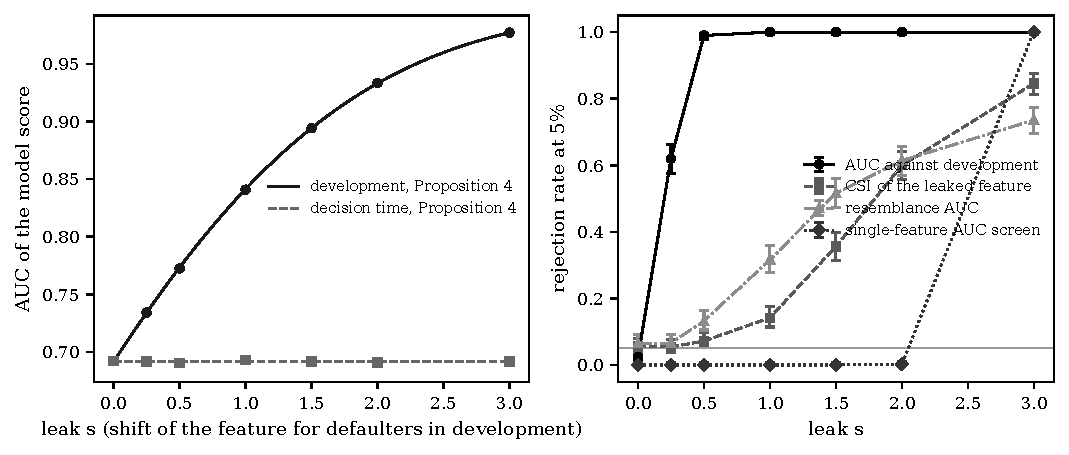
\includegraphics[width=\textwidth]{figures/fig-planted-leak.pdf}
\caption{The leak planted by the engine generator, with 150 defaulters and 4,850 survivors per sample: left, the simulated mean AUC in development and at decision time against the leak $s$ with the closed forms of Proposition~\ref{prop:leakauc}; right, the percentage of 500 repetitions in which each detector rejects at 5\%, with Wilson intervals.}
\label{fig:planted-leak}
\end{figure}

\begin{table*}[htbp]
\centering
\small
\caption{The leak planted by the engine generator (150 defaulters and 4,850 survivors per sample, 500 repetitions per level): simulated mean AUC in development and at decision time beside the closed forms of Proposition 4, and the percentage of repetitions in which each detector rejects at 5\%: the AUC-against-development test, the characteristic stability index of the leaked feature, the resemblance AUC and the single-feature AUC screen at its default threshold of 0.95.}
\label{tab:planted-leak}
\fitwidth{%
\begin{tabular}{rrrrrrrrr}
\toprule
Leak $s$ & Dev. AUC sim. & Dev. AUC Prop. & Current AUC sim. & Current AUC Prop. & AUC test power & CSI power & Resemblance power & Single-feature flag \\
\midrule
0 & 0.692 & 0.691 & 0.692 & 0.691 & 2.4 & 5.6 & 6.6 & 0.0 \\
0.25 & 0.734 & 0.734 & 0.692 & 0.691 & 62.0 & 5.4 & 6.6 & 0.0 \\
0.5 & 0.772 & 0.773 & 0.691 & 0.691 & 99.0 & 7.2 & 13.2 & 0.0 \\
1 & 0.841 & 0.841 & 0.693 & 0.691 & 100.0 & 14.2 & 31.6 & 0.0 \\
1.5 & 0.894 & 0.894 & 0.692 & 0.691 & 100.0 & 35.6 & 51.6 & 0.0 \\
2 & 0.933 & 0.933 & 0.691 & 0.691 & 100.0 & 60.0 & 61.4 & 0.2 \\
3 & 0.977 & 0.977 & 0.692 & 0.691 & 100.0 & 84.6 & 73.6 & 100.0 \\
\bottomrule
\end{tabular}%
}
\end{table*}


Table~\ref{tab:planted-leak} and Figure~\ref{fig:planted-leak} show what the engine's detectors see of a leak that is present in development and absent at decision time. The closed forms of Proposition~\ref{prop:leakauc} reproduce the simulated mean AUC at every level (the largest standardised difference over the seven levels is \nv{e3.zmax}, within three), and the development AUC is inflated by \nv{e3.s1.0.infl} at $s=1$ while the decision-time AUC does not move. The AUC-against-development test, which compares the current AUC with its development value, rejects in \nv{e3.s0.25.auc_test}\% of the repetitions at $s=0.25$, \nv{e3.s0.5.auc_test}\% at $s=0.5$ and \nv{e3.s1.0.auc_test}\% from $s=1$ upward, and at $s=0$ in \nv{e3.s0.0.auc_test}\%. The stability index of the leaked feature rejects in \nv{e3.s0.5.csi_test}\% at $s=0.5$, \nv{e3.s1.0.csi_test}\% at $s=1$ and \nv{e3.s2.0.csi_test}\% at $s=2$, against \nv{e3.s0.0.csi_test}\% under no leak. The committed document of the case, with \nv{c22.reps} repetitions per level, gives \nv{c22.csi.0.5}\%, \nv{c22.csi.1}\% and \nv{c22.csi.2}\% for the index at $s=0.5$, 1 and 2 and \nv{c22.auc.0.25}\%, \nv{c22.auc.0.5}\% and \nv{c22.auc.1}\% for the test against development at $s=0.25$, 0.5 and 1, which agrees with these rates; its null rate for the test against development is \nv{c22.auc.0}\% against \nv{e3.s0.0.auc_test}\% here (Wilson interval \nv{e3.s0.0.auc_lo} to \nv{e3.s0.0.auc_hi}\%), a difference of \nv{c22.null.diff} points (pooled two-proportion $z=\nv{c22.null.z}$, $p=\nv{c22.null.p}$) that the repetitions do not allow for and that this paper does not explain. Both rates are below the nominal 5\%, so the test is conservative at $s=0$ in these set-ups; at the leaked levels the two sets of rates agree. The resemblance AUC rejects in \nv{e3.s1.0.resemblance_flag}\% at $s=1$. The single-feature screen flags the leaked feature in \nv{e3.s1.0.single_feature_flag}\% at $s=1$ and in \nv{e3.s2.0.single_feature_flag}\% at $s=2$, because the feature alone has an AUC of \nv{e3.s1.0.feat} and \nv{e3.s2.0.feat}, below the threshold of 0.95; at $s=3$ the AUC of the feature is \nv{e3.s3.0.feat} and the screen flags it in \nv{e3.s3.0.single_feature_flag}\%. The sixth prediction holds: the test against development has a power of \nv{e3.s0.5.auc_test}\% at $s=0.5$ and the two feature-based detectors have \nv{e3.s1.0.csi_test}\% and \nv{e3.s1.0.single_feature_flag}\% at $s=1$. The explanation is Proposition~\ref{prop:psi}: the index of the leaked feature, \nv{th.psi.1.0.binned_chi2_form} at $s=1$ by the theory and \nv{th.psi.1.0.engine_psi} by the engine's exact value, is below the level of \nv{th.psi.null} that two samples of 5,000 rows produce by chance. The leak is a drop of discrimination out of time, not a drift of the feature.

\subsection{A random split against the out-of-time cohort}

\begin{figure}[htbp]
\centering
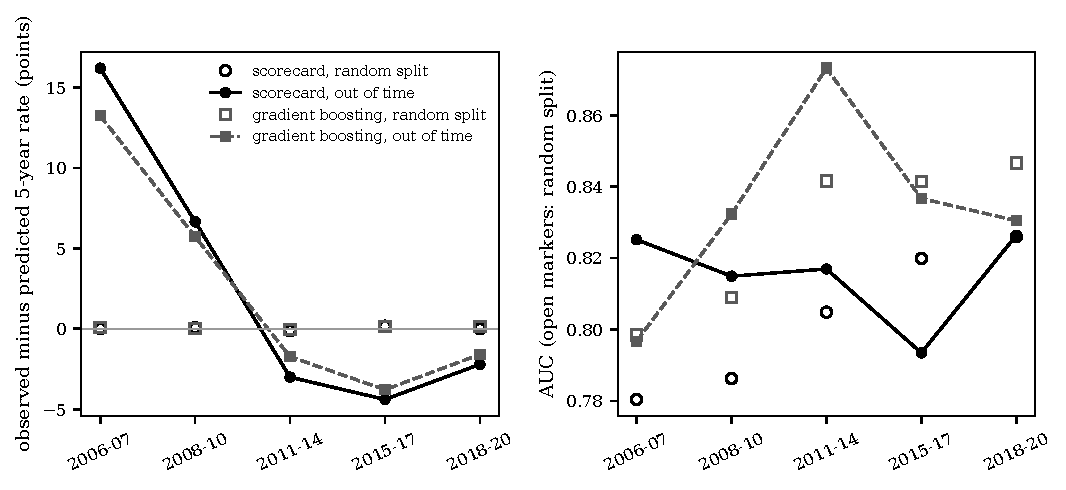
\includegraphics[width=\textwidth]{figures/fig-out-of-time.pdf}
\caption{For the five cohorts of the SBA 7(a) loans, left, the observed minus the predicted 5-year charge-off rate in percentage points of the scorecard and of the gradient-boosting rung on a random sample of the training window and on the out-of-time cohort; right, the AUC of the same rungs on the two samples (open markers: random split).}
\label{fig:out-of-time}
\end{figure}

\begin{table*}[htbp]
\centering
\small
\caption{Two estimates of the same fitted models on the SBA 7(a) loans of C03: a random sample of the training window's own loans that neither the fit nor the calibration used (rand.), and the declared out-of-time cohort at the 5-year mark of each vintage (OOT). The gap is the observed minus the predicted 5-year charge-off rate in percentage points; the columns are the WoE scorecard (Score.) and the monotone gradient-boosting rung (GBM), and the training window of each cohort is in the table of splits.}
\label{tab:out-of-time}
\fitwidth{%
\begin{tabular}{lrrrrrrrrr}
\toprule
Cohort & Window loans & \shortstack{Score.\\AUC rand.} & \shortstack{Score.\\AUC OOT} & \shortstack{Score.\\gap rand.} & \shortstack{Score.\\gap OOT} & \shortstack{GBM\\AUC rand.} & \shortstack{GBM\\AUC OOT} & \shortstack{GBM\\gap rand.} & \shortstack{GBM\\gap OOT} \\
\midrule
FY2006-07 & 330,682 & 0.780 & 0.825 & 0.0 & +16.2 & 0.799 & 0.797 & +0.1 & +13.2 \\
FY2008-10 & 413,083 & 0.786 & 0.815 & +0.1 & +6.6 & 0.809 & 0.832 & 0.0 & +5.7 \\
FY2011-14 & 627,594 & 0.805 & 0.817 & $-$0.1 & $-$3.0 & 0.842 & 0.873 & $-$0.1 & $-$1.7 \\
FY2015-17 & 900,254 & 0.820 & 0.793 & +0.2 & $-$4.4 & 0.841 & 0.837 & +0.1 & $-$3.8 \\
FY2018-20 & 1,024,597 & 0.826 & 0.826 & 0.0 & $-$2.2 & 0.847 & 0.830 & +0.1 & $-$1.6 \\
\bottomrule
\end{tabular}%
}
\end{table*}


Table~\ref{tab:out-of-time} and Figure~\ref{fig:out-of-time} compare, for the same fitted models, a random sample of the training window that the fit and the calibration did not read with the declared out-of-time cohort. On the random sample the level of the scorecard is right in every cohort: the gap between observed and predicted 5-year rates is between \nv{e4.2011-14.sc.random_gap} and \nv{e4.2015-17.sc.random_gap} points, within \nv{e4.maxz} binomial standard errors of the 60,000-loan sample at the window rate of each cohort (\nv{e4.sed.lo} to \nv{e4.sed.hi} points; \nv{e4.holdse} points is the largest value that a binomial standard error of this sample can take), for the scorecard and for the gradient-boosting rung. On the out-of-time cohort the gap is \nv{e4.2006-07.sc.oot_gap} points for the cohort of fiscal years 2006 and 2007, whose observed 5-year rate is \nv{e4.2006-07.rate_oot}\% against \nv{e4.2006-07.rate_random}\% in the window, \nv{e4.2008-10.sc.oot_gap} for 2008 to 2010, \nv{e4.2011-14.sc.oot_gap} for 2011 to 2014, \nv{e4.2015-17.sc.oot_gap} for 2015 to 2017 and \nv{e4.2018-20.sc.oot_gap} for 2018 to 2020; the gradient-boosting rung has gaps of the same sign and a smaller size, namely \nv{e4.2006-07.gbm.oot_gap}, \nv{e4.2008-10.gbm.oot_gap}, \nv{e4.2011-14.gbm.oot_gap}, \nv{e4.2015-17.gbm.oot_gap} and \nv{e4.2018-20.gbm.oot_gap}, which is below 2 points for the cohorts \nv{h8.failed}. A random split cannot see the shift of level, because the window it samples has the level of the window. The eighth prediction, applied to both rungs, does not hold: the random gap is below one point in \nv{h8.rand} of \nv{h8.cells} cohort and rung cells, and the out-of-time gap is at least two points in \nv{h8.oot} of \nv{h8.cells}, the exceptions being the two gradient-boosting cells named above. The scorecard clears the rule in every cohort, with a smallest out-of-time gap of \nv{c03.mingap} points, a value that the committed documents of the case already held. The AUC behaves differently and is not systematically optimistic: the out-of-time AUC of the scorecard is above the random-split AUC for the first three cohorts (\nv{e4.2006-07.sc.oot_auc} against \nv{e4.2006-07.sc.random_auc} for the first) and below it for 2015 to 2017 (\nv{e4.2015-17.sc.oot_auc} against \nv{e4.2015-17.sc.random_auc}). What the declared cohort measures, and the random split does not, is the level. The run reproduces the committed out-of-time AUC of the scorecard of every cohort to within \nv{e4.maxrepdiff}.

\subsection{Cross-validation with preprocessing outside the folds}

\begin{figure}[htbp]
\centering
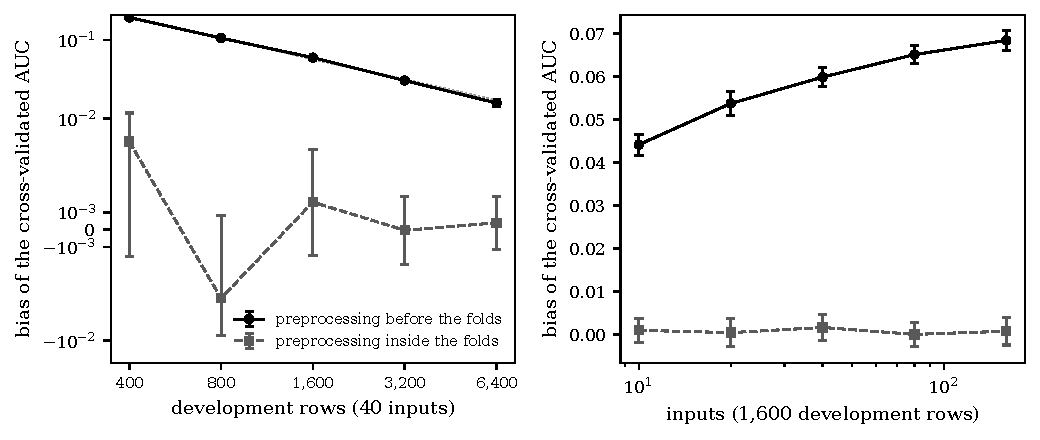
\includegraphics[width=\textwidth]{figures/fig-cv-scaling.pdf}
\caption{Bias of the five-fold AUC against the mean reference AUC of the fold models for the WoE scorecard on planted data, with preprocessing fitted inside each training fold (squares) or on all development rows before the folds (circles); left, against the number of development rows at 40 inputs on a symmetric logarithmic scale, with the fitted power law; right, against the number of inputs at 1,600 rows.}
\label{fig:cv-scaling}
\end{figure}

\begin{table}[htbp]
\centering
\small
\caption{Bias of five-fold cross-validated AUC against the mean reference AUC of the fold models for the WoE scorecard on planted data (five informative inputs, the rest noise), 100 repetitions per row, with the preprocessing fitted inside each training fold or on all development rows before the folds; the 95\% half-widths are over repetitions.}
\label{tab:cv-scaling}
\fitwidth{%
\begin{tabular}{rrrr}
\toprule
Development rows & Inputs & Preprocessing inside the folds & Preprocessing before the folds \\
\midrule
400 & 40 & $+0.005\pm0.007$ & $+0.194\pm0.005$ \\
800 & 40 & $-0.004\pm0.005$ & $+0.106\pm0.003$ \\
1,600 & 40 & $+0.002\pm0.003$ & $+0.060\pm0.002$ \\
3,200 & 40 & $0.000\pm0.002$ & $+0.031\pm0.002$ \\
6,400 & 40 & $+0.000\pm0.002$ & $+0.016\pm0.001$ \\
1,600 & 10 & $+0.001\pm0.003$ & $+0.044\pm0.002$ \\
1,600 & 20 & $+0.000\pm0.003$ & $+0.054\pm0.003$ \\
1,600 & 80 & $0.000\pm0.003$ & $+0.065\pm0.002$ \\
1,600 & 160 & $+0.001\pm0.003$ & $+0.068\pm0.002$ \\
\bottomrule
\end{tabular}%
}
\end{table}


Table~\ref{tab:cv-scaling} and Figure~\ref{fig:cv-scaling} give the bias of the five-fold AUC. With the preprocessing fitted inside each fold the bias is within the noise at all nine combinations (from \nv{e5.n800.p40.in} to \nv{e5.n400.p40.in}). With the preprocessing before the folds the bias is \nv{e5.n400.p40.out} at 400 development rows and falls to \nv{e5.n6400.p40.out} at 6,400, with a power-law slope of $-\nv{e5.exp}\pm\nv{e5.expse}$, from which the range of the exponent in the conjecture was read, so that the fit does not test it; at 1,600 rows it rises from \nv{e5.n1600.p10.out} at 10 inputs to \nv{e5.n1600.p160.out} at 160 and flattens. The ninth prediction, applied to both models on all three data sets, does not hold: the outside-fold bias is positive in \nv{h9.pos} of 6 pairs of data set and model and the inside-fold bias is null in \nv{h9.null} of 6. The exceptions are the logit on the card holders before the folds (\nv{tw.l.cvpre.bias}$\,\pm\,$\nv{tw.l.cvpre.ci}, not inflated) and the logit on the planted data inside the folds (\nv{syn.l.cvin.bias}$\,\pm\,$\nv{syn.l.cvin.ci}, a small negative bias); for the scorecard the contrast holds on all three data sets. The conjecture is consistent with the evidence and is not proved.

\subsection{Whether each prediction held}

Table~\ref{tab:hypotheses} gives the outcome of every prediction, applying each rule to every cell that the paper reports. Of the nine, \nv{h.held.word} held (H1, H3, H4, H5, H6 and H7) and \nv{h.notheld.word} did not (H2, H8 and H9). The second did not: on the card holders the screen with holdout labels does not raise the AUC beyond the noise (\nv{tw.w.scr.bias}$\,\pm\,$\nv{tw.w.scr.ci}), so that the claim that every label-reading step inflates the estimate is established for the weight of evidence and for the fit on everything and is not established for the screen on this data set. The eighth did not: the out-of-time gap of the gradient-boosting rung is below 2 points in two of the five cohorts, so that the contrast between a random split and the declared cohort holds at the size of two points for the scorecard and not for a second model. The ninth did not: the logit is not inflated by preprocessing before the folds on the card holders and is slightly negative inside the folds on the planted data, so that the contrast holds for the scorecard on every data set and not for the logit on every one. The third prediction held, and its holding is a limit of the claim that leaks inflate the estimate: the leaks through inputs only did not. The seventh held with a largest standardised difference of \nv{e3.zmax}, and the closed forms of the theory are reproduced by the generator. The sixth and the eighth were set with committed values of the cases in view (Section~\ref{sec:experimental-design}), so that the sixth is a reproduction of those values by new runs and the eighth a check that the scorecard clears a threshold placed at them. Two readings follow. The three failures concern the direction and size of an effect for one step, one rung or one model on one data set, and they do not touch the propositions, which make no claim about the screen on any data set, about the gradient-boosting rung or about the logit. The holding of the third prediction and of the scorecard rows of the ninth says that the rule on inputs and the rule on folds differ in kind: the first has no measurable cost in the estimate, and the second is the largest cost measured.
